\usetikzlibrary{arrows.meta,chains}

\begin{frame}{layering}
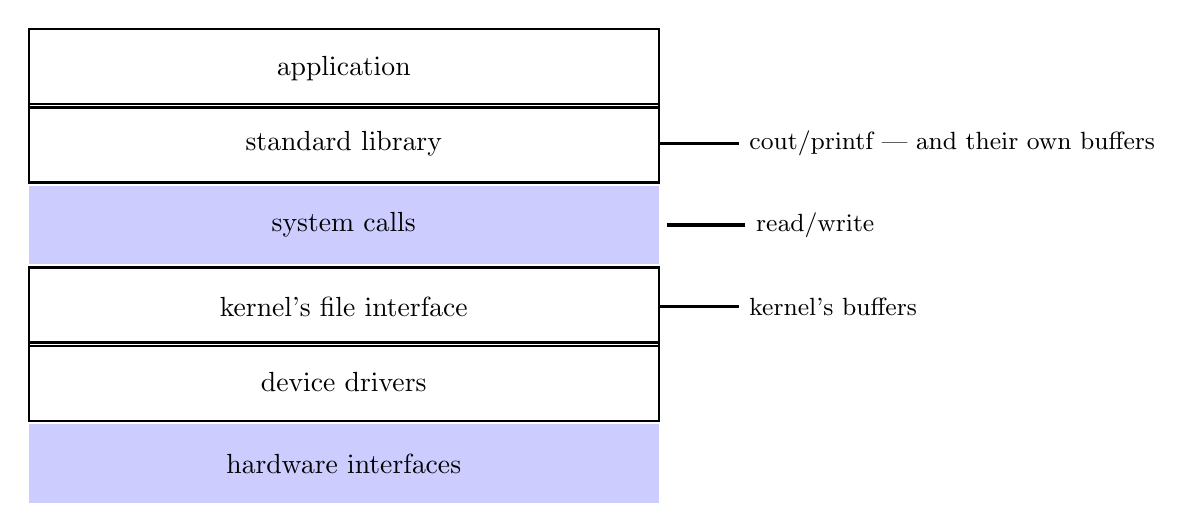
\begin{tikzpicture}
\tikzset{
    box/.style={draw,thick,minimum width=8cm,minimum height=1cm},
    thin box/.style={fill=blue!20,minimum width=8cm,minimum height=1cm,outer sep=1mm},
}
\begin{scope}[start chain=going below,node distance=-.75mm,every node/.style={on chain}]
\node[box] (application) {application};
\node[box] (library) {standard library};
\node[thin box] (syscalls) {system calls};
\node[box] (kernel file) {kernel's file interface};
\node[box] (device driver) {device drivers};
\node[thin box] (hardware) {hardware interfaces};
\end{scope}
\draw[very thick] (kernel file.east) -- ++(1cm,0cm) node[right,font=\small] {kernel's buffers};
\draw[very thick] (syscalls.east) -- ++(1cm,0cm) node[right,font=\small] {read/write};
\draw[very thick] (library.east) -- ++(1cm,0cm) node[right,font=\small] {cout/printf --- \myemph{and their own buffers}};
\end{tikzpicture}
\end{frame}

\begin{frame}{why the extra layer}
    \begin{itemize}
        \item better (but more complex to implement) interface:
            \begin{itemize}
            \item read line 
            \item formatted input (scanf, cin into integer, etc.)
            \item formatted output
            \end{itemize}
        \item less system calls (bigger reads/writes) sometimes faster
            \begin{itemize}
            \item buffering can combine multiple in/out library calls into one system call
            \end{itemize}
        \item more portable interface
            \begin{itemize}
            \item cin, printf, etc. defined by C and C++ standards
            \end{itemize}
    \end{itemize}
\end{frame}
